\documentclass[12pt]{article}
\usepackage{latexsym,amssymb,amsmath} % for \Box, \mathbb, split, etc.
% \usepackage[]{showkeys} % shows label names
\usepackage{cite} % sorts citation numbers appropriately
\usepackage{path}
\usepackage{url}
\usepackage{verbatim}
\usepackage{graphicx}
\usepackage{array}
\usepackage{multirow}

% horizontal margins: 1.0 + 6.5 + 1.0 = 8.5
\setlength{\oddsidemargin}{0.0in}
\setlength{\textwidth}{6.5in}
% vertical margins: 1.0 + 9.0 + 1.0 = 11.0
\setlength{\topmargin}{0.0in}
\setlength{\headheight}{12pt}
\setlength{\headsep}{13pt}
\setlength{\textheight}{625pt}
\setlength{\footskip}{24pt}

\renewcommand{\textfraction}{0.10}
\renewcommand{\topfraction}{0.85}
\renewcommand{\bottomfraction}{0.85}
\renewcommand{\floatpagefraction}{0.90}
\usepackage{graphicx}
\usepackage{wrapfig}
\usepackage{lscape}
\usepackage{rotating}
\usepackage{epstopdf}
\makeatletter
\setlength{\arraycolsep}{2\p@} % make spaces around "=" in eqnarray smaller
\makeatother

% change equation, table, figure numbers to be counted inside a section:
\numberwithin{equation}{section}
\numberwithin{table}{section}
\numberwithin{figure}{section}

% begin of personal macros
\newcommand{\half}{{\textstyle \frac{1}{2}}}
\newcommand{\eps}{\varepsilon}
\newcommand{\myth}{\vartheta}
\newcommand{\myphi}{\varphi}
\usepackage[utf8]{inputenc}

% Default fixed font does not support bold face
\DeclareFixedFont{\ttb}{T1}{txtt}{bx}{n}{8} % for bold
\DeclareFixedFont{\ttm}{T1}{txtt}{m}{n}{8}  % for normal

% Custom colors
\usepackage{color}
\definecolor{deepblue}{rgb}{0,0,0.5}
\definecolor{deepred}{rgb}{0.6,0,0}
\definecolor{deepgreen}{rgb}{0,0.5,0}
\definecolor{backcolour}{rgb}{0.96,0.96,0.96}

\usepackage{listings}

% cpp style for highlighting
\newcommand\cppstyle{\lstset{
		language=C++,
        basicstyle=\tiny\ttfamily,
		keywordstyle=\color{blue}\ttfamily,
		stringstyle=\color{red}\ttfamily,
		commentstyle=\color{green}\ttfamily,
		morecomment=[l][\color{magenta}]{\#},
		frame=tb,                         % Any extra options here
showstringspaces=false,            % 
backgroundcolor=\color{backcolour}
}}


% cpp environment
\lstnewenvironment{cpp}[1][]
{
	\cppstyle
	\lstset{#1}
}
{}

% cpp for external files
\newcommand\cppexternal[2][]{{
		\cppstyle
		\lstinputlisting[#1]{#2}}}

% cpp for inline
\newcommand\cppinline[1]{{\cppstyle\lstinline!#1!}}

\newcommand{\IN}{\mathbb{N}}
\newcommand{\IZ}{\mathbb{Z}}
\newcommand{\IQ}{\mathbb{Q}}
\newcommand{\IR}{\mathbb{R}}
\newcommand{\IC}{\mathbb{C}}
\newcommand{\Real}[1]{\mathrm{Re}\left({#1}\right)}
\newcommand{\Imag}[1]{\mathrm{Im}\left({#1}\right)}
\usepackage{booktabs}
\usepackage{caption}
\usepackage{float}
\usepackage{titlesec}
\usepackage{capt-of}
%dashed line
\usepackage{array}
\usepackage{arydshln}
\setlength\dashlinedash{0.2pt}
\setlength\dashlinegap{1.5pt}
\setlength\arrayrulewidth{0.3pt}

%Widows & Orphans & Penalties

\widowpenalty500
\clubpenalty500
\clubpenalty=9996
\exhyphenpenalty=50 %for line-breaking at an explicit hyphen
\brokenpenalty=4991
\predisplaypenalty=10000
\postdisplaypenalty=1549
\displaywidowpenalty=1602
\floatingpenalty = 20000
\usepackage[T1]{fontenc}
\usepackage{fontspec}
\setmainfont[Scale=0.85, Ligatures={Required,Common,Contextual,TeX}]{TeX Gyre Schola} % Incredible font inside latex


\newcommand{\norm}[2]{\|{#1}\|_{{}_{#2}}}
\newcommand{\abs}[1]{\left|{#1}\right|}
\newcommand{\ip}[2]{\left\langle {#1}, {#2} \right\rangle}
\newcommand{\der}[2]{\frac{\partial {#1}}{\partial {#2}}}
\newcommand{\dder}[2]{\frac{\partial^2 {#1}}{\partial {#2}^2}}
\usepackage{enumitem}
\newcommand{\nn}{\mathbf{n}}
\newcommand{\xx}{\mathbf{x}}
\newcommand{\uu}{\mathbf{u}}
\usepackage{tikz}
\usetikzlibrary{arrows}
\usetikzlibrary{positioning}
\usepackage{titlesec}
\newcommand{\junk}[1]{{}}
\usepackage{sectsty}
\usepackage{xcolor}

\newcommand\MyBox[2]{
	\fbox{\lower0.75cm
		\vbox to 1.7cm{\vfil
			\hbox to 1.7cm{\hfil\parbox{1.4cm}{#1\\#2}\hfil}
			\vfil}%
	}%
}

\makeatletter
\renewcommand*\env@matrix[1][\arraystretch]{%
	\edef\arraystretch{#1}%
	\hskip -\arraycolsep
	\let\@ifnextchar\new@ifnextchar
	\array{*\c@MaxMatrixCols c}}
\makeatother

\makeatletter
\renewcommand*\env@matrix[1][*\c@MaxMatrixCols c]{%
	\hskip -\arraycolsep
	\let\@ifnextchar\new@ifnextchar
	\array{#1}}
\makeatother

\definecolor{darkblue}{rgb}{0,0,0.4}
\usepackage[colorlinks = true,
linkcolor = darkblue,
urlcolor  = darkblue,
citecolor = darkblue,
anchorcolor = darkblue]{hyperref}
% set two lengths for the includegraphics commands used to import the plots:
\newlength{\fwtwo} \setlength{\fwtwo}{0.45\textwidth}
% end of personal macros

\begin{document}
\DeclareGraphicsExtensions{.jpg}

\begin{center}
\textsc{\Huge Multi-core Programming} \\[2pt]
	\textsc{\Large Assignment 2}\\
	\vspace{0.5cm}
  Ali Gholami \\[6pt]
  Department of Computer Engineering \& Information Technology\\
  Amirkabir University of Technology  \\[6pt]
  \def\UrlFont{\em}
  \url{https://aligholamee.github.io}\\
\href{mailto:aligholami7596@gmail.com}{\textit{aligholami7596@gmail.com}}
\end{center}

\begin{abstract}
A tree has many analogies in real life, and turns out that it has influenced a wide area of machine learning, covering both classification and regression. In decision analysis, a decision tree can be used to visually and explicitly represent decisions and decision making. As the name goes, it uses a tree-like model of decisions. Though a commonly used tool in data mining for deriving a strategy to reach a particular goal, its also widely used in machine learning, which will be the main focus of this article.
\end{abstract} 

\subparagraph{Keywords.} \textit{Heterogeneous Programming, OpenMP, C Programming, C++ Programming, Parallelization, Multi-thread Programming.}

\section{Matrix Multiplication}
\subsection{What's the goal?}
In this assignment, we'll be parallelizing the matrix multiplication using \textit{OpenMP}. The goal is to speed up the matrix multiplication by implementing the parallelization in two axis (\textit{1D} \& \textit{2D}). Below the serial code for the matrix multiplication. Sources for this assignment is available in the repository merged with this report.

\begin{cpp}
		void multiply(DataSet dataSet){
			int i, j, k, sum;
			for(i = 0; i < dataSet.n; i++){
				for(j = 0; j < dataSet.p; j++){
					sum = 0;
					for(k = 0; k < dataSet.m; k++){
						sum += dataSet.A[i * dataSet.m + k] * dataSet.B[k * dataSet.p + j];
					}
					dataSet.C[i * dataSet.p + j] = sum;
				}
			}
		}
\end{cpp}

\subsection{1D Parallelization}
The following figures are provided from the problem description by \textit{Dr. Ahmad Siavashi}. Each of the highlighted areas show a job for a thread. Figure 1.1 shows how the multiplication is done by each thread.
\begin{figure}[!h]\centering
	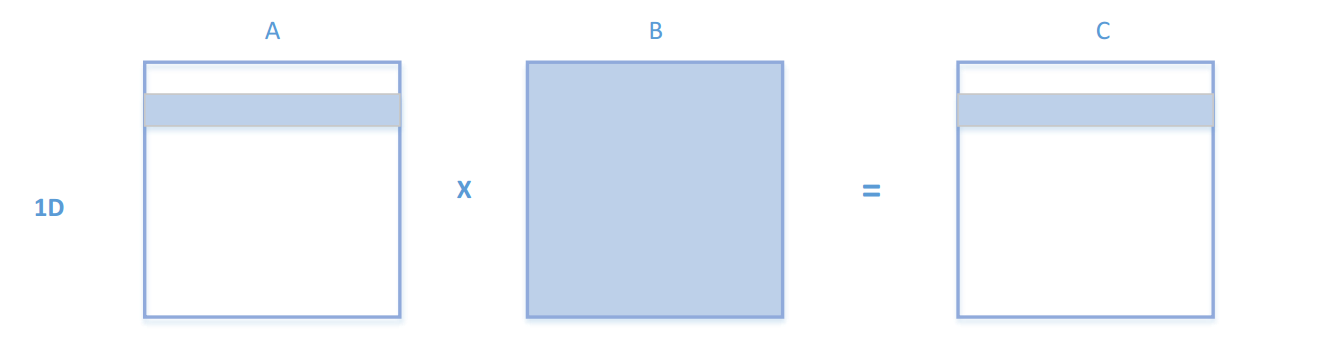
\includegraphics[width=0.8\textwidth]{one_dimensional.png}
	\caption{Matrix Multiplication Parallelization on Horizontal Axis.}
	\label{figsolplot}
\end{figure}\\
Assuming each \textit{integer} as 4 bytes, we'll be filling the table 1.1 using the average time computed after 6 times of running the program.
\begin{thebibliography}{999}
	
	\bibitem{cross_validation}
	Prashant Gupta,
	\emph{Cross-Validation in Machine Learning}.
	Towards Data Science,
	Jun 5, 2017.

	
\end{thebibliography}
\end{document}